% !TEX encoding = UTF-8 Unicode
\documentclass[10pt,aspectratio=169,]{beamer}
\setbeamercovered{transparent=10}
\usetheme[
%  showheader,
%  red,
  purple,
%  gray,
%  graytitle,
  colorblocks,
%  noframetitlerule,
]{Verona}

\usepackage[T1]{fontenc}
\usepackage[utf8]{inputenc}
\usepackage{lipsum}
\usepackage{tikz}
\usetikzlibrary{fadings}
\usepackage{multimedia}
\usepackage{media9}
\graphicspath{{figuras/}}
\usepackage{mathtools}
\usepackage{dsfont}
\usepackage{eurosym}
%
%\setbeamertemplate{sections/subsections in toc}[ball]
\usepackage{listings}
\usepackage{caption}
\usepackage{subcaption}
\usefonttheme{professionalfonts}
\def\mathfamilydefault{\rmdefault}
\usepackage{amsmath}
\usepackage{multirow}
\usepackage{booktabs}
\usepackage{bm}
\setbeamertemplate{section in toc}{\hspace*{1em}\inserttocsectionnumber.~\inserttocsection\par}
\setbeamertemplate{subsection in toc}{\hspace*{2em}\inserttocsectionnumber.\inserttocsubsectionnumber.~\inserttocsubsection\par}
\setbeamerfont{subsection in toc}{size=\small}
%\AtBeginSection[]{%
%	\begin{frame}%
%		\frametitle{Outline}%
%		\textbf{\tableofcontents[currentsection]} %
%	\end{frame}%
%}



\newcommand{\sectionpagemod}{
	\begingroup
    \beamertemplateshadingbackground{structure.fg!90}{structure.fg}
    \setbeamercolor{section page}{fg=white}
    \setbeamertemplate{section page}{
    \begin{tikzpicture}                                             %edit this tikzpicture to customize the appearance of the section heading
        \node[overlay] {\insertsectionhead};
    \end{tikzpicture}
    }
    \frame{\vfill
	\begin{center}{\textbf{\Huge \sectionpage}}\end{center}
	\vfill}
    \endgroup
}

\newcommand{\subsectionpagemod}{
	\begingroup
    \beamertemplateshadingbackground{structure.fg!90}{structure.fg}
    \setbeamercolor{subsection page}{fg=white}
    \setbeamertemplate{subsection page}{
    \begin{tikzpicture}                                             %edit this tikzpicture to customize the appearance of the section heading
        \node[overlay] {\insertsubsectionhead};
    \end{tikzpicture}
    }
    \frame{\vfill
	\begin{center}{\Huge \color{white}\subsectionpage}\end{center}
	\vfill}
    \endgroup
}

\title{Implementación de una blockchain \mbox{resistente} a ataques criptográficos cuánticos}
\subtitle{Trabajo Fin de Grado}
\author[]{\textbf {Autor\\ María Victoria Granados Pozo\\ \footnotesize Directores\\ Gabriel Maciá Fernández\\ Francisco Javier Lobillo Borrero}}
\institute[]{Doble grado de Ingeniería Informática y Matemáticas\\
Universidad de Granada}
\date{\today}
\titlegraphic[width=4cm]{logoUGR.pdf}{}
%\titlegraphic[width=5cm]{logo.png}{}




\begin{document}

\maketitle

%%% define code
\defverbatim[colored]\lstI{
	\begin{lstlisting}[language=C++,basicstyle=\ttfamily,keywordstyle=\color{red}]
	int main() {
	// Define variables at the beginning
	// of the block, as in C:
	CStash intStash, stringStash;
	int i;
	char* cp;
	ifstream in;
	string line;
	[...]
	\end{lstlisting}
}
%%%%%%%%%%%%%%%%%%%%%%%%%%%%%%%%
% ----------- FRAME ------------
%%%%%%%%%%%%%%%%%%%%%%%%%%%%%%%%
\begin{frame}%
	\frametitle{Contenidos}%
	\textbf{\tableofcontents} %
\end{frame}

\section{Introducción}
\sectionpagemod

%El contexto en el que surge este proyecto, es una sociedad digitalizada donde los dispositivos digitales comportan la mayor parte de las actividades. De esta forma cabe pensar como de seguras son esas actividades destacando las actividades económicas. Ya que el objetivo principal del proyecto es evitar que un sistema blockchain sea vulnerable a futuros atáques cuánticos.
\begin{frame}[c]{Motivación}
	\begin{figure}
		\centering
		
\includegraphics[height=4cm]{logo.png}
	\end{figure}
\end{frame}

%Los avances tecnologícos deben venir acompañados de mecanismos que aporten seguridad. Los tres pilares de la seguridad informática  se denominan CIA que son, confidencialidad que garantiza que un tercero no pueda acceder a los datos, la integridad que mantiene la exactitud de los datos, esto es, que no haya modificaciones durante su envío, y la disponibilidad de los datos en todo momento.

\begin{frame}[c]{Motivación}
	\begin{figure}
		\centering
		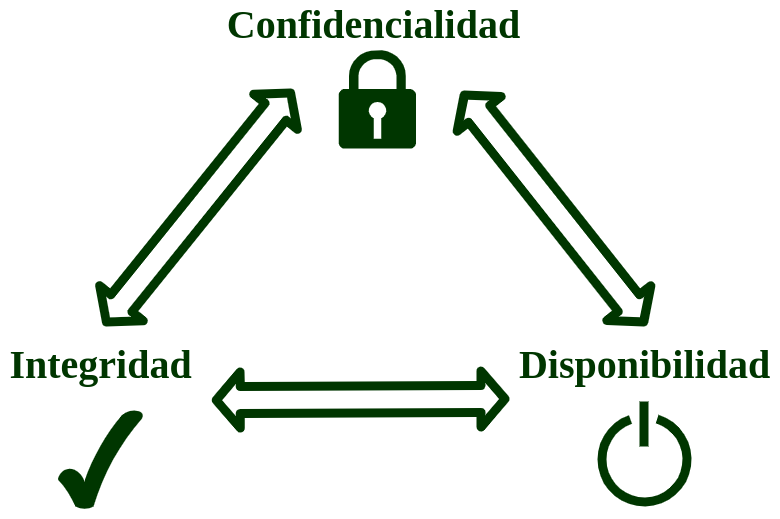
\includegraphics[height=4cm]{CIA.png}
		\caption{Pilares de la seguridad informática}
	\end{figure}
\end{frame}

%Para llevar a cabo el objetivo del proyecto ha sido necesario realizar dos tareas. Por un lado, la implementación del algoritmo UOV en python, esto son las funciones para la generación de las claves pública y privadas, y las funciones para la firma y validación de la misma, ya que no existen bibliotecas de python que permitan trabajar con matrices y cuerpos finitos también se ha implementado la aritmética del cuerpo finito de 128 elementos específica para el algoritmo UOV. Por otro lado, para comprobar el funcionamiento del algoritmo y aumentar la seguridad de la cadena de bloques se ha integrado en la blockchain de ARK, modificando los algoritmo de firma y verificación.
\begin{frame}[c]{Objetivos}
	\begin{exampleblock}{Implementación del algoritmo UOV}
		Funciones propias del algoritmo y aritmética del cuerpo finito de $2^7$ elementos.
	\end{exampleblock}

	\begin{exampleblock}{Integración del algoritmo UOV}
		Modificación del algoritmo de firma de la blockchain de ARK por el algoritmo UOV.
	\end{exampleblock}
\end{frame}

\section{Contenidos teóricos}
\sectionpagemod
%Es un nuevo paradigma de la informática que basa sus principios en la teoría cuántica.
\subsection*{Computación cuántica}
\subsectionpagemod
%Dichos principios son la superposición cuántica describe como una particula puede estar en diferentes estados al mismo tiempo, el entrelazamiento cuántico que dos particulas se conectan si han interactuado una vez y el teletransporte cuantico que se envia la informacion por el espacio sin viajar a traves de el.

\begin{frame}[c]{Propiedades computación cuántica}
	\begin{itemize}
		\item Superposición cuántica.
		\item Entrelazamiento cuántico.
		\item Teletransporte cuántico.
	\end{itemize}
\end{frame}

%Lo que aporta una mayor capacidad de cómputo, pero que a poca escala los computadores clásicos siguen siendo mejores.
\begin{frame}[c]{Comparativa computación cuántica y clásica}
	\begin{figure}
		\centering
		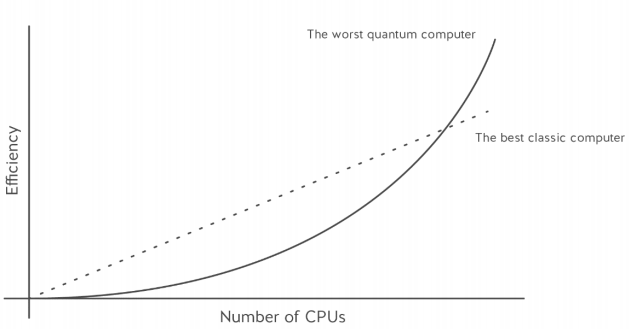
\includegraphics[height=4cm]{comp_clasica_cuantica.png}
	\end{figure}
\end{frame}



\subsection*{Blockchain}
\subsectionpagemod


% El algoritmo UOV, o algoritmo de aceite y vinagre desequilibrado es un algoritmo de firma digital. Para la creación de la firma y validarla es necesario resolver un sistema con m ecuaciones y n variables, que es un problema NP-duro. Como no existe un algoritmo de resolución de sistemas de ecuaciones multivariados eficiente en ordenadores cuánticos, la firma permanecera segura. Debido a que las operaciones son sumas y productos se requieren bajos recursos hardware.
\subsection*{Algoritmo UOV\large\textit{(Unbalance Oil and Vinegar)}}
\subsectionpagemod

\begin{frame}[c]{Ventajas del algoritmo UOV}
	\begin{itemize}
		\item Problema NP-duro.
		\item No se conoce un algoritmo eficiente para la resolución de sistemas multivariados en un ordenador cuántico.
		\item Simplicidad de las operaciones.
		\item Requiere bajos recursos \textit{hardware}.
	\end{itemize}
\end{frame}

%El esquema de la firma UOV utiliza la función unidireccional P de F sub 2 elevado a r de tamaño n en F sub 2 elevado a r de tamaño m, función cuadrática multivariante en $n = m + v$ variables. Esta función se puede descomponer como F compuesto con T, donde T va de F sub 2 elevado a r de tamaño n en F sub 2 elevado a r de tamaño n es linear invertible, y F va de F sub 2 elevado a r de tamaño n en F sub 2 elevado a r de tamaño m  función cuadrática cuyas $m$ componentes son de la forma... donde alpha y beta se toman aleatoriamente en F sub 2 siendo alpha un vector de matrices triangulares superiores. Se toma así alpha para que sea más eficiente sin afectar a la seguridad. Las primeras $v$ variables de x son las variables vinagres y las $m$ variables restantes son las variables aceite.

\begin{frame}[c]{Esquema UOV}
	$$\mathcal{P}: \mathds{F}_{2^r}^n \rightarrow \mathds{F}_{2^r}^m$$\\
	\vfill
	$\mathcal{P} = \mathcal{F} \circ \mathcal{T}$, donde $\mathcal{T}: \mathds{F}_{2^r}^n \rightarrow \mathds{F}_{2^r}^n$  y $\mathcal{F}: \mathds{F}_{2^r}^n \rightarrow \mathds{F}_{2^r}^m$\\
	\vfill
	\begin{equation}\label{eq:fun}
		f_k(x) = \sum_{i=1}^v \sum_{j=i}^n \alpha_{i,j,k} x_i x_j + \sum_{i=1}^n \beta_{i,k} x_i
	\end{equation}
	donde $\alpha_{i,j,k}$ y $\beta_{i,k}$ se toman aleatoriamente en $\mathds{F}_2$ siendo $\left(\alpha_{i,j,k}\right)_{\begin{subarray}{l}{1\leqslant i \leqslant v }\\ {1 \leqslant j \leqslant n}\end{subarray}}$ un vector de matrices triangulares superiores.
\end{frame}





\section{Planificación y presupuesto}
\sectionpagemod
\begin{frame}[c]{Diagrama de Gantt}
	\begin{figure}
		\centering
		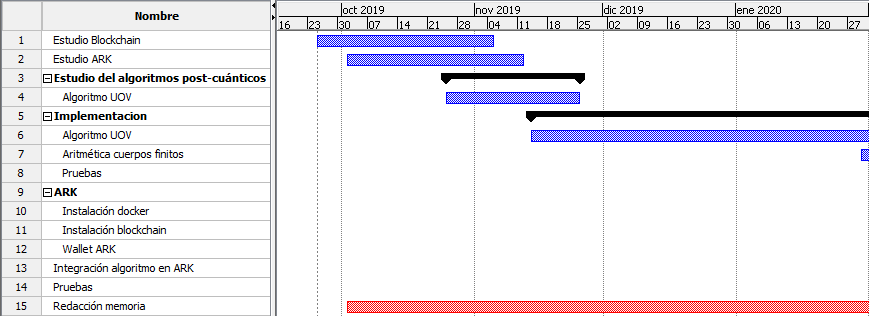
\includegraphics[height=4cm]{Gantt_1.png}
	\end{figure}
\end{frame}

\begin{frame}[c]{Diagrama de Gantt}
	\begin{figure}
		\centering
		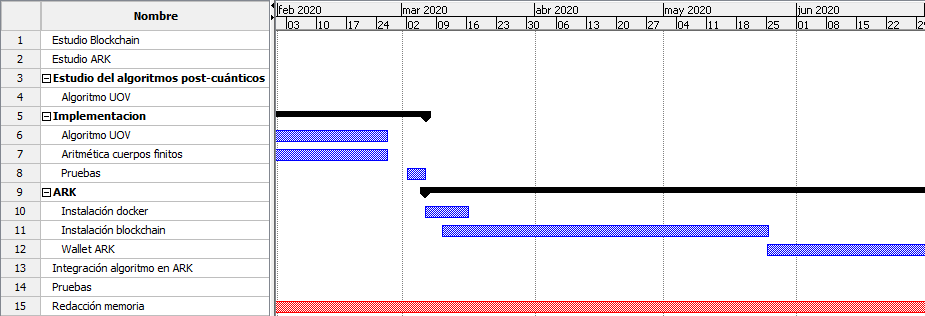
\includegraphics[height=4cm]{Gantt_2.png}
	\end{figure}
\end{frame}

\begin{frame}[c]{Diagrama de Gantt}
	\begin{figure}
		\centering
		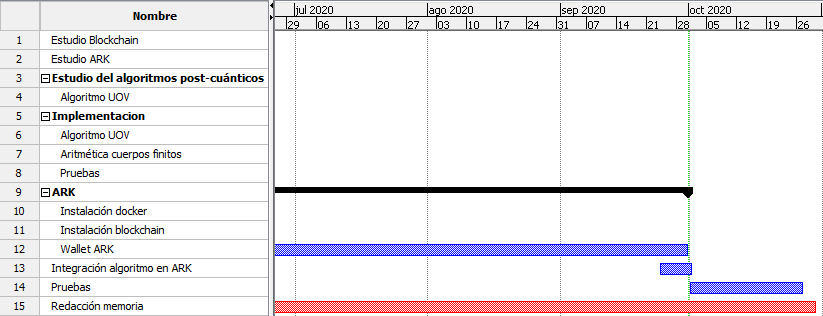
\includegraphics[height=4cm]{Gantt_3.png}
	\end{figure}
\end{frame}

\begin{frame}[c]{Presupuesto desglosado}
	\begin{table}[H]
		\begin{center}
		\centering
		\begin{tabular}{p{0.6\linewidth} p {0.2\linewidth}}
			\textbf{Tipo de costes} & \textbf{Cantidad} \\
			\toprule
			Recursos humanos tutores & 4.830\euro\\[0.5ex]
			Recursos humanos alumna & 10.720\euro\\[0.5ex]
			Indirectos & 755,24\euro\\[0.5ex]
			Directos & 210,40\euro\\[0.5ex]
			Viajes & 22\euro\\[0.5ex]
			Gastos imprevistos & 826,88\euro\\[0.5ex]
			\bottomrule
			TOTAL (\euro) & 17.364,52\euro\\
		\end{tabular}
		\end{center}
		\label{tab:coste-total}
	\end{table}
\end{frame}

\section{Diseño}
\sectionpagemod
\begin{frame}[c]{Diagrama de bloques del prototipo}
	\begin{figure}
		\centering
		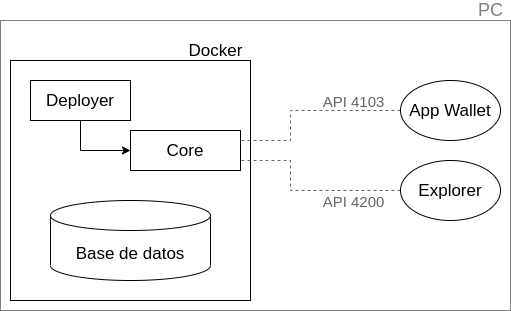
\includegraphics[height=4cm]{diagrama_bloquesARK.png}
		\caption{Diagrama de bloques prototipo}
	\end{figure}
\end{frame}


\section{Demostración práctica}
\sectionpagemod

%Por último veamos las conclusiones y futuras lineas de investigación
\section{Conclusiones e investigaciones futuras}
\sectionpagemod
\begin{frame}[c]{Conclusiones}

\end{frame}
%De cara al futuro de podría trabajar con la base de datos en lugar de mantener la información en fichero \texttt{json} independientes. Además se podría integrar la blockchain modificada en otra no tiene porque de ARK, para hacerla más segura, esto se podría hacer por las propiedades de ARK blockchain.
\begin{frame}[c]{Trabajos futuros}
	\begin{itemize}
		\item Trabajar con la base de datos.
		\item Integrar la \textit{blockchain} ARK modificada en otra cadena de bloques.
	\end{itemize}
\end{frame}



% Thank you page
\beamertemplateshadingbackground{structure.fg!90}{structure.fg}
\begin{frame}[plain]
	\vfill
	\centering
	{
		\centering \Huge \color{white} !`Gracias por su atención!\\[10pt]
	}
	\vfill
\end{frame}

\end{document}


